\section{Evaluation}\label{sec:eval}

\subsection{Generalisation}
\label{Generalisation} 

\begin{table*}\centering
\ra{1.3}
\begin{tabular}{@{}lrrrrrrrrrrrrrrr@{}}\toprule
& \multicolumn{3}{c}{RENI} & \phantom{ab}& \multicolumn{3}{c}{RENI++} &
\phantom{ab} & \multicolumn{3}{c}{SH} &
\phantom{ab} & \multicolumn{3}{c}{SG}\\
\cmidrule{2-4} \cmidrule{6-8} \cmidrule{10-12} \cmidrule{14-16}
D & PSNR$\uparrow$ & SSIM$\uparrow$ & LPIPS$\downarrow$ && PSNR$\uparrow$ & SSIM$\uparrow$ & LPIPS$\downarrow$ && PSNR$\uparrow$ & SSIM$\uparrow$ & LPIPS$\downarrow$ && PSNR$\uparrow$ & SSIM$\uparrow$ & LPIPS$\downarrow$\\ \midrule
27 & 
17.02 & \textbf{0.40} & 0.75 &&
\textbf{18.02} & 0.39 & \textbf{0.62} &&
15.00 & 0.33 & 0.79 && 
17.67 & 0.35 & 0.80 \\
108 & 
19.58 & 0.45 & 0.75 && 
\textbf{20.87} & \textbf{0.49} & \textbf{0.56} &&
17.88 & 0.38 & 0.79 && 
19.27 & 0.41 & 0.70 \\
147 & 
19.97 & 0.46 & 0.74 && 
\textbf{21.13} & \textbf{0.51} & \textbf{0.55} && 
18.23 & 0.40 & 0.77 && 
19.81 & 0.43 & 0.67 \\ 
300 & 
20.47 & 0.48 & 0.73 && 
\textbf{22.10} & \textbf{0.55} & \textbf{0.52} && 
19.15 & 0.45 & 0.74 && 
20.24 & 0.46 & 0.61 \\
\bottomrule
\end{tabular}
\caption{The mean PSNR, SSIM, and LPIPS scores for tone-mapped LDR images when fitting to the test set for increasing latent dimensions. Where an exact dimensionality comparison is not possible for SG, e.g. in the $D=27$ and $D=147$ cases, we bias in favour of SG with a $D=30$ and $D=150$ respectively.}
\label{tab:comparison_PSNR_SSIM_LPIPS}
\end{table*}

We begin by evaluating the generalisation ability of RENI++ when approximating unseen environments. We compare against original RENI, SH and SG and explore how generalisation performance varies as a function of latent code dimension. We consider RGB spherical harmonics of order 2, 5, 6 and 9 equal to latent code dimension $D = 3 \times N$ for $N=9, 36, 49, 100$. Since SG requires a dimensionality that is a multiple of 6, where $D$ is not a multiple of 6, we bias in SGs favour by using the next multiple, i.e.~$\lceil D/6 \rceil \cdot 6$. We re-implemented within Nerfstudio open-source implementations of per-pixel environment map fitting for SG provided by \cite{li_inverse_2020} and \cite{charlmersgitSphericalHarmonics2022} for SH and used these to fit our models within the same environment as RENI++. As shown in Figure \ref{fig:comparison}, RENI++ can capture higher frequency detail than SH, SG and the original RENI implementation, is less dominated by high-value pixels and can reproduce accurate HDR values. A comparison of the mean PSNR across the test set images for increasing latent code dimensionality is shown in Table \ref{tab:comparison_PSNR_SSIM_LPIPS}.

\begin{figure*}
    \centering
    \makebox[\textwidth]{%
        \begin{tikzpicture}
            \node (img) {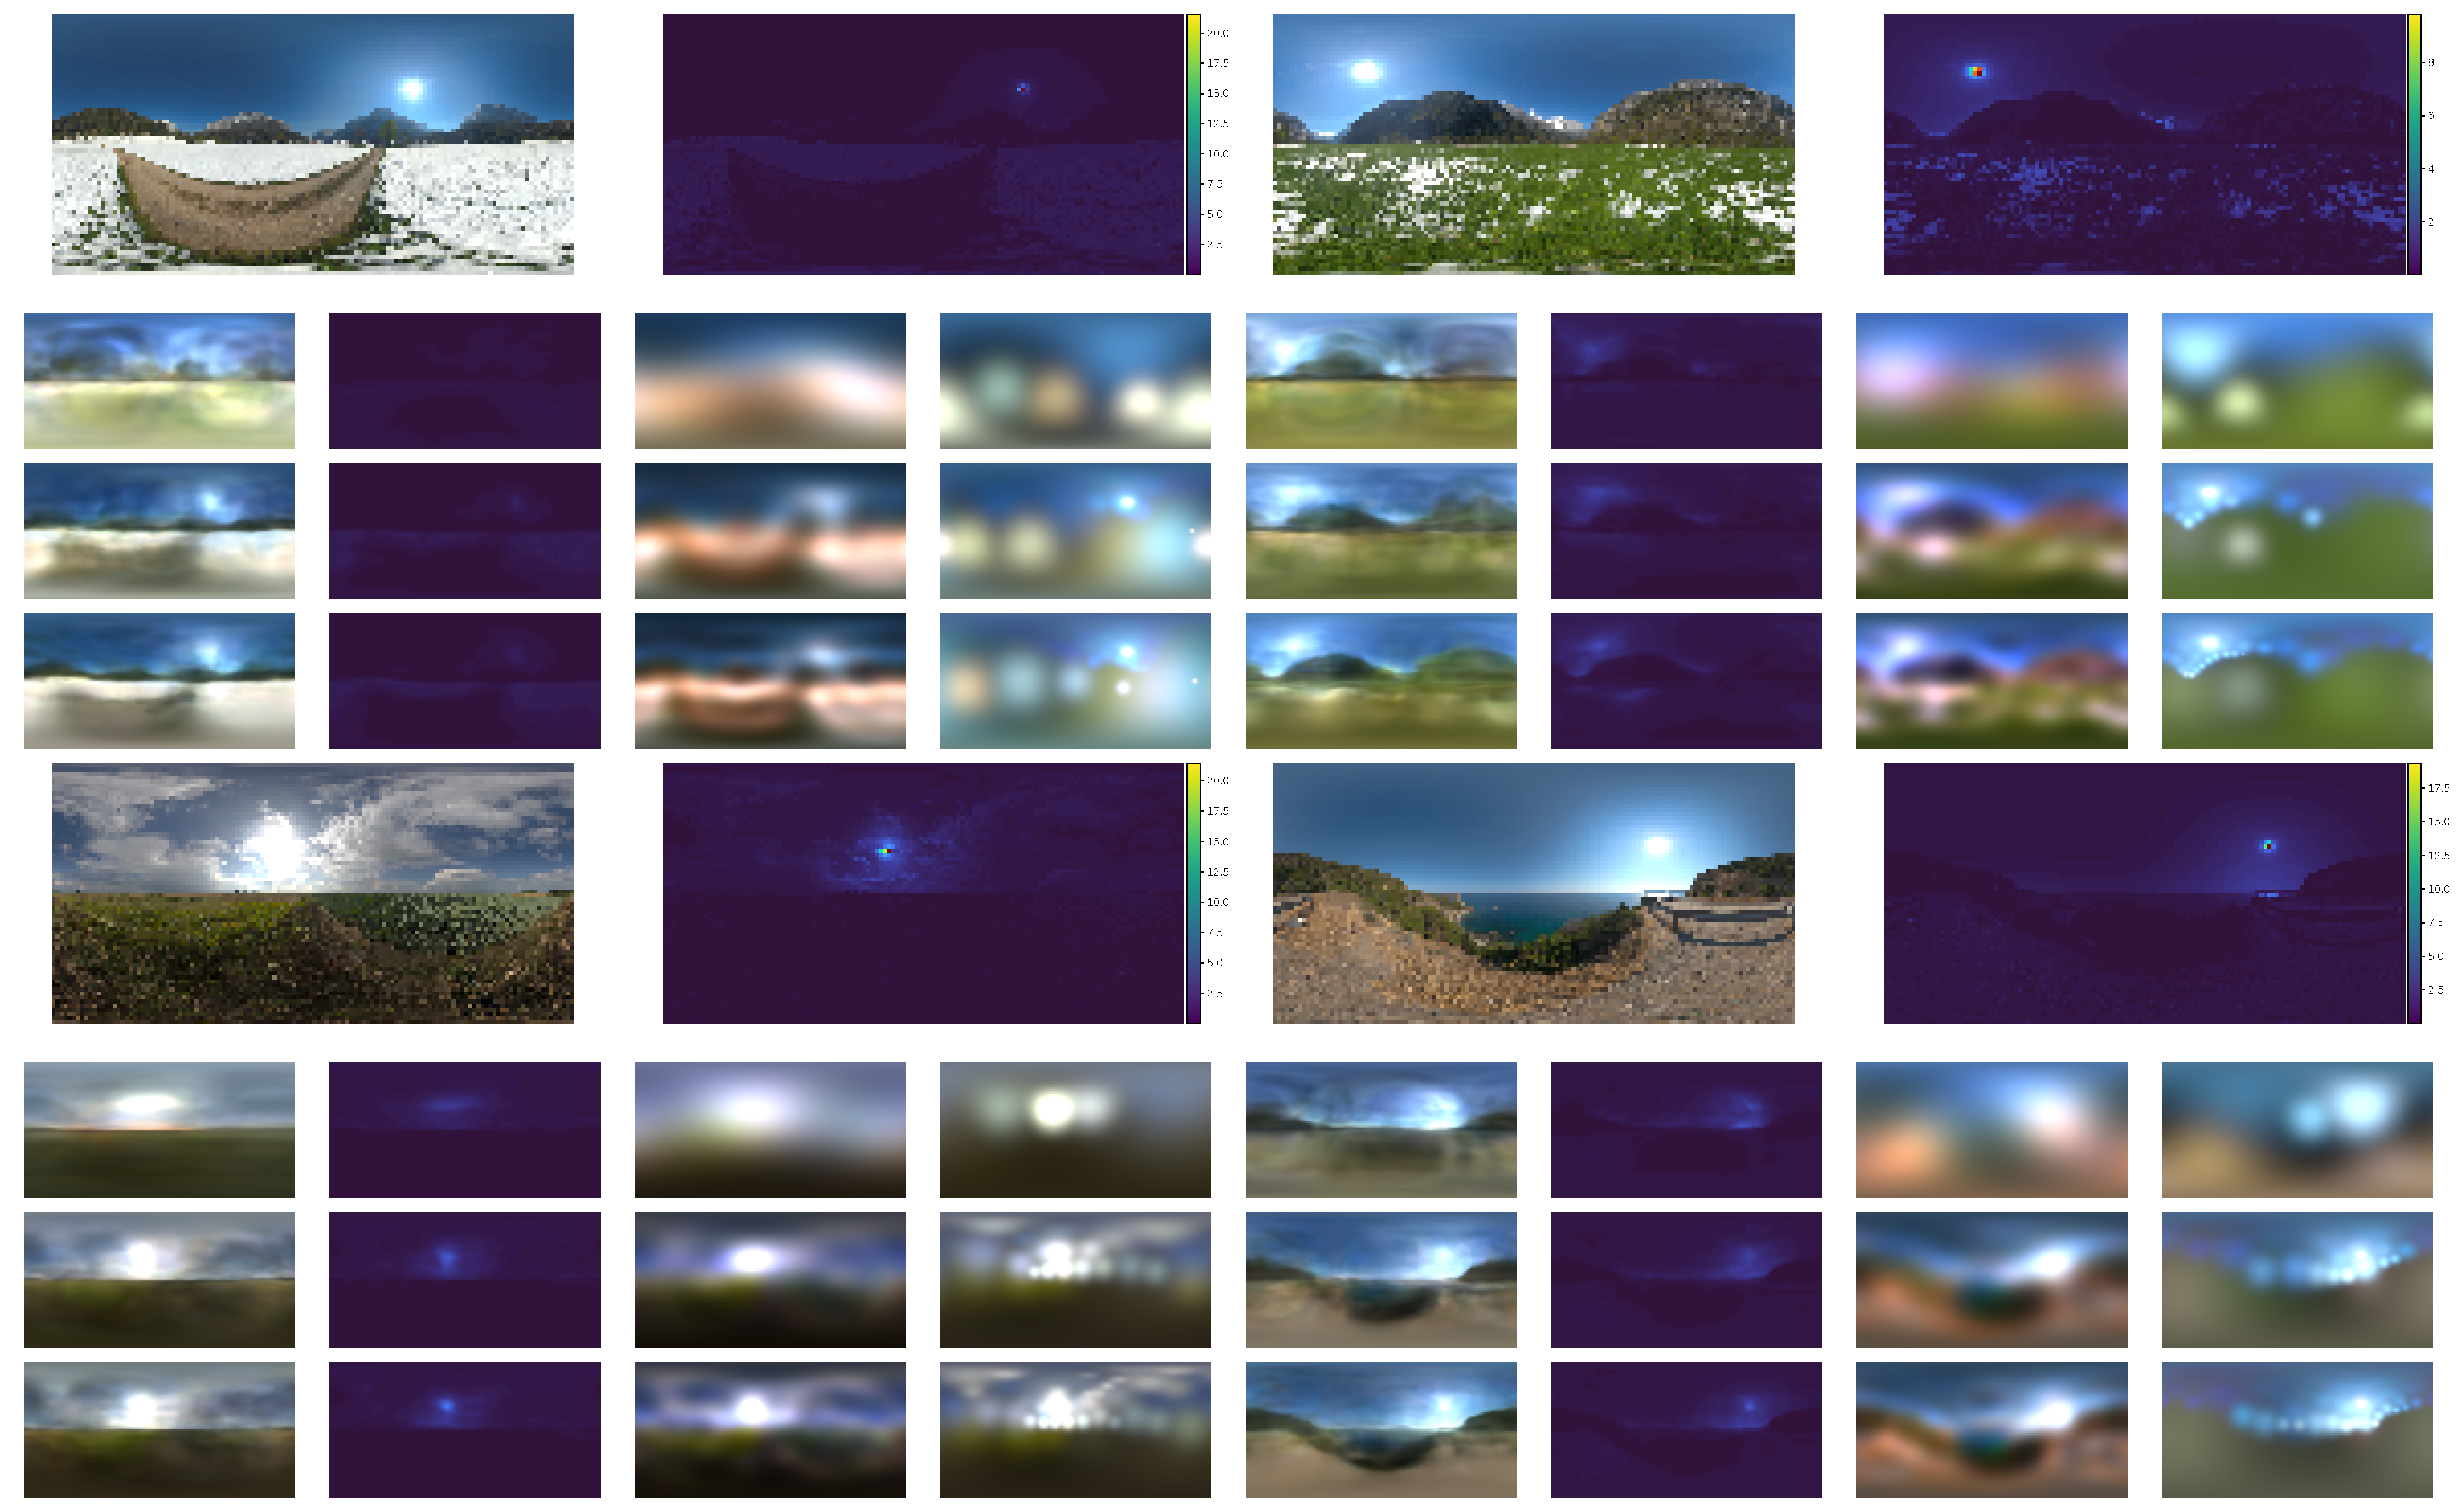
\includegraphics[width=1.00\textwidth]{Figures/comparison.pdf}};
            \node at (-9.1, 4.5) [rotate=90] {\tiny Ground Truth};
            \node at (-9.1, -1.0) [rotate=90] {\tiny Ground Truth};
            \node at (-9.1, 2.75) [rotate=90] {\tiny 27};
            \node at (-9.1, 1.65) [rotate=90] {\tiny 147};
            \node at (-9.1, 0.55) [rotate=90] {\tiny 300};
            \node at (-9.1, -2.8) [rotate=90] {\tiny 27};
            \node at (-9.1, -3.9) [rotate=90] {\tiny 147};
            \node at (-9.1, -5.0) [rotate=90] {\tiny 300};
            \node at (-6.8, 3.4) {\tiny RENI++};
            \node at (-3.4, 3.4) {\tiny SH};
            \node at (-1.1, 3.4) {\tiny SG};
            \node at (2.3, 3.4) {\tiny RENI++};
            \node at (5.65, 3.4) {\tiny SH};
            \node at (7.9, 3.4) {\tiny SG};
            \node at (-6.8, -2.15) {\tiny RENI++};
            \node at (-3.4, -2.15) {\tiny SH};
            \node at (-1.1, -2.15) {\tiny SG};
            \node at (2.3, -2.15) {\tiny RENI++};
            \node at (5.65, -2.15) {\tiny SH};
            \node at (7.9, -2.15) {\tiny SG};
        \end{tikzpicture}
    }
    \caption{Generalisation to unseen images with latent code dimensions, $D = 3N$ for $N=9, 36, 49$ and for SH of equal dimensionality (orders 2, 6, and 9). SG results are with dimensionality $D = 30, 150, 300$. Log-scale heat maps for ground truth and RENI++ are also shown.}
    \label{fig:comparison}
\end{figure*}

\subsection{Latent Space Interpolation}
As shown in Figure \ref{fig:Interpolations}, linear interpolations between codes result in smooth transitions between images and plausible natural environments for all intermediate latent codes showing how RENI++ encodes a meaningful internal representation of natural illumination.


\begin{figure*}[!ht]
    \centering
    \begin{tikzpicture}
    \node (img) {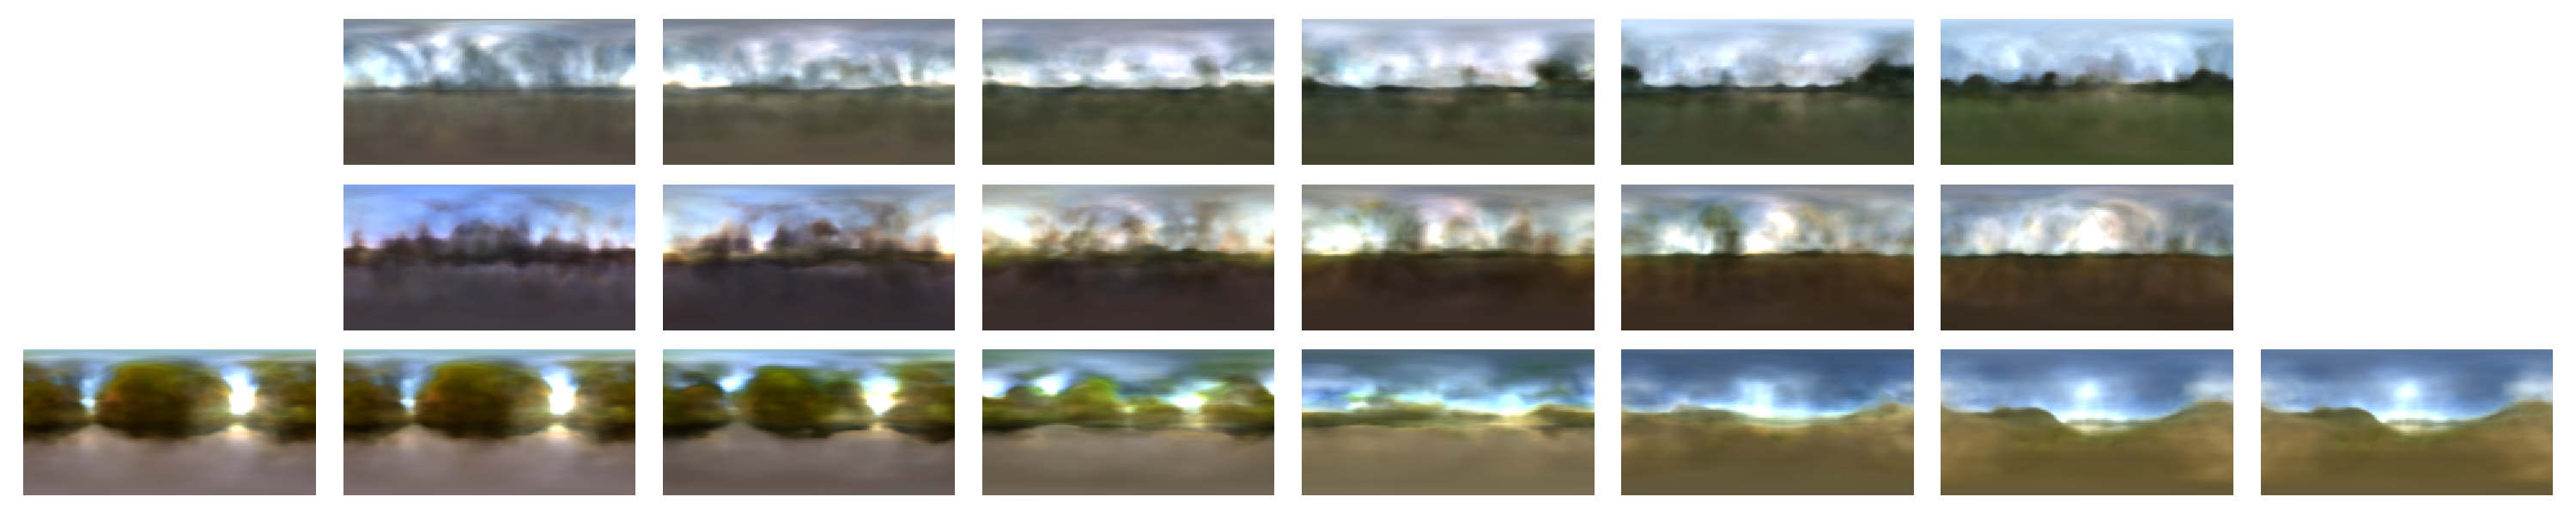
\includegraphics[width=0.98\textwidth]{Figures/interpolations_and_random_samples.pdf}};
    \end{tikzpicture}
    \caption{Interpolation results for RENI++ with latent code dimension of $D = 300$. Rows 1 and 2 show interpolations between two random latent codes, and row 3 shows an interpolation between two training images with the ground-truth images shown.}
    \label{fig:Interpolations}
\end{figure*}

\subsection{Environment Completion}

Any picture of a natural scene contains cues about the surrounding environment that the scene was captured in, such as likely sun locations and possible environmental content. If RENI++ is only provided with a small portion of the complete environment map in its loss at test time, RENI++ can hallucinate plausible completions of the environment. As shown in Figure \ref{fig:outpainting}, RENI++ makes sensible estimations about the possible colours and shapes of land and sky and often predicts quite accurate sun locations despite the sun being outside the image crop.

\begin{figure*}[h]
    \centering
    \begin{tikzpicture}
    \node (img) {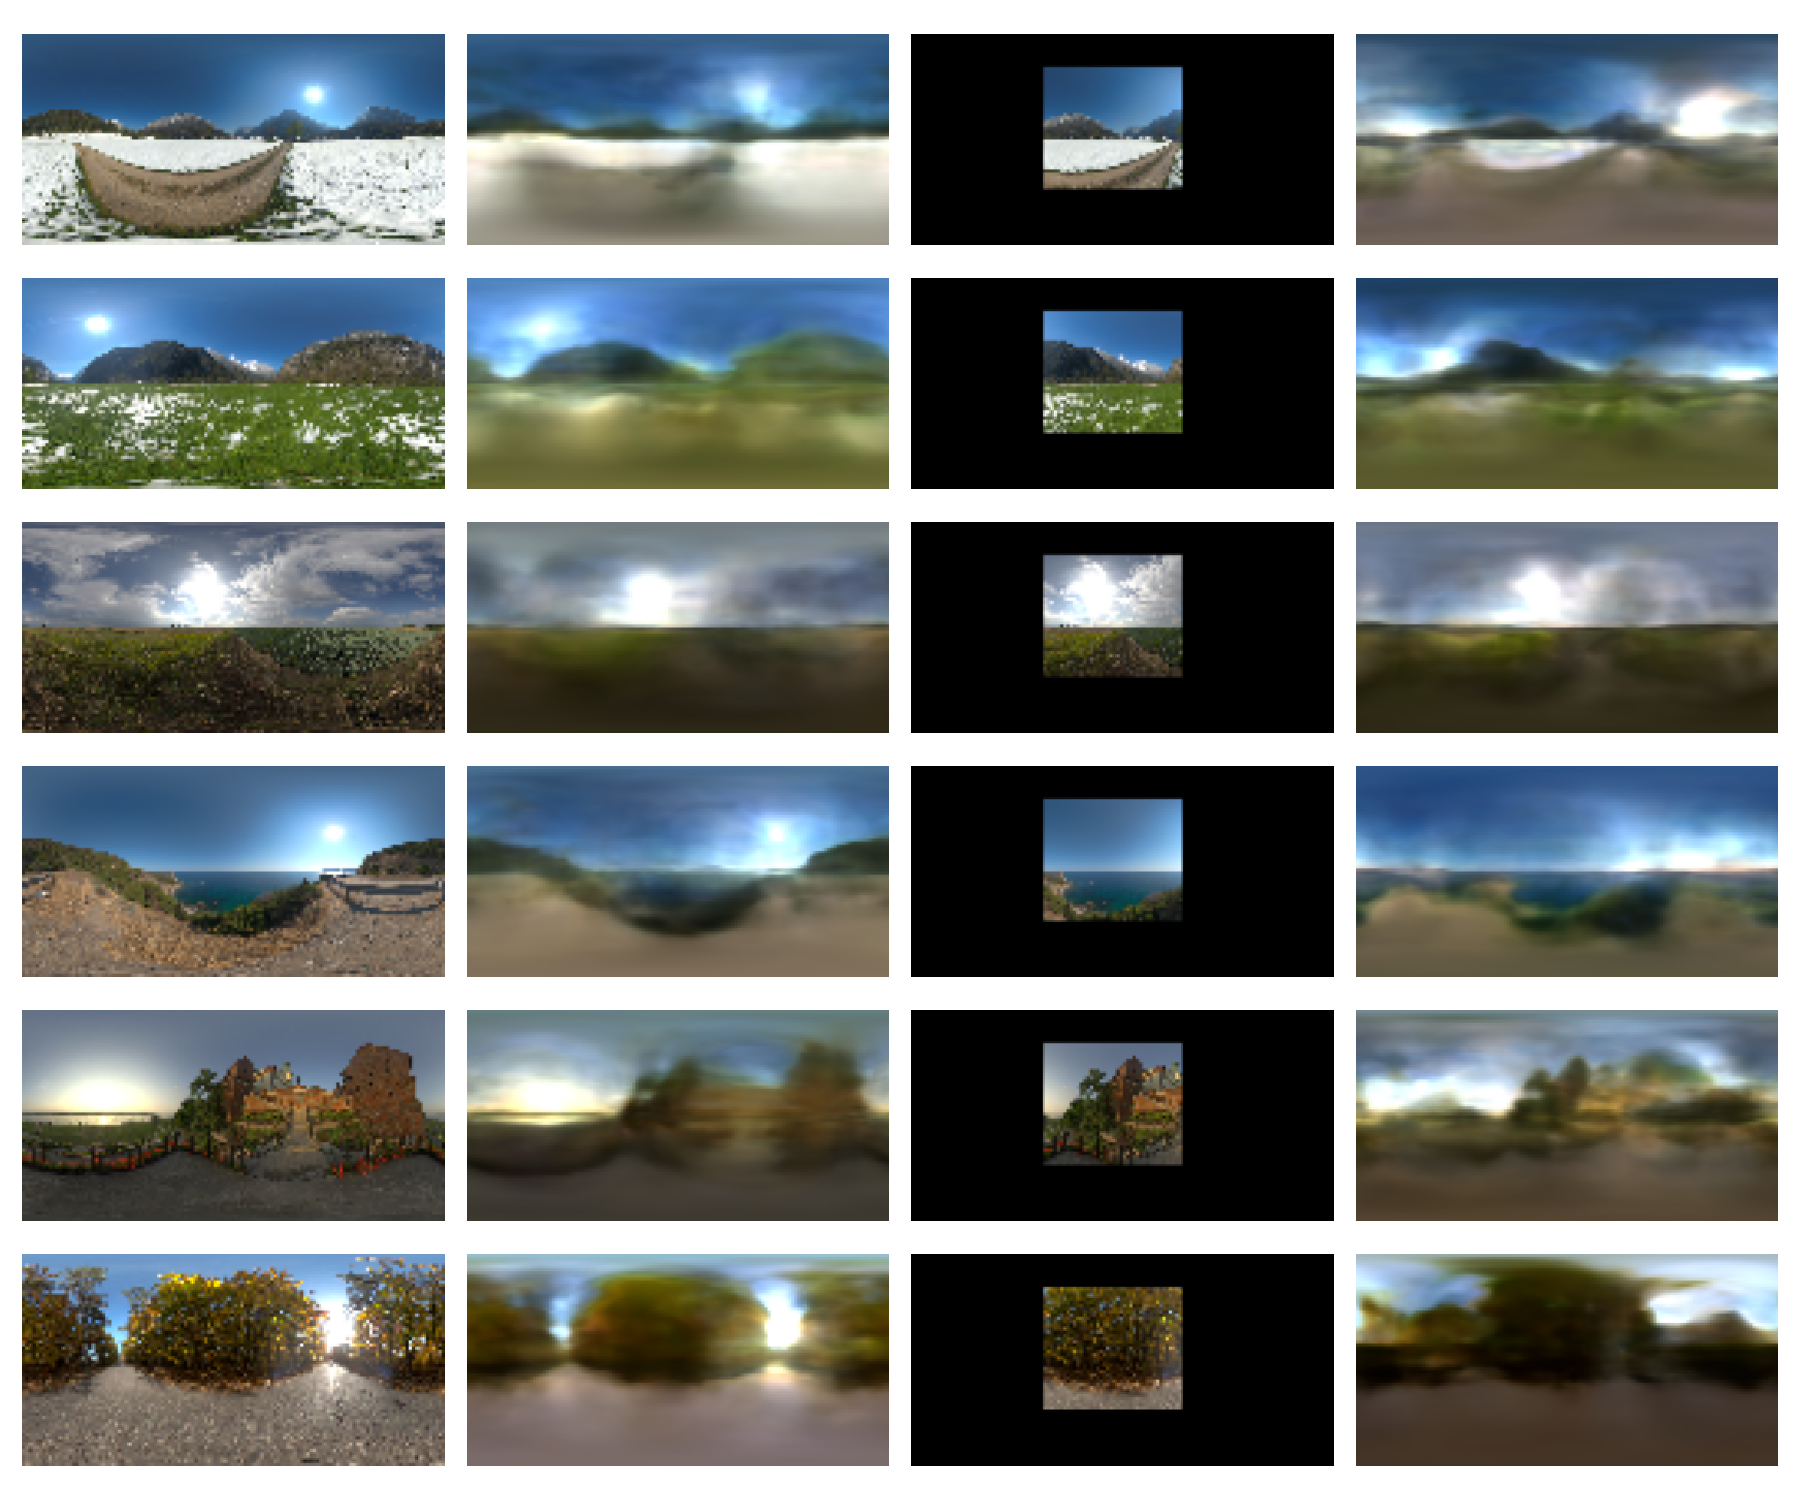
\includegraphics[width=0.98\textwidth]{Figures/outpainting.pdf}};
    \node at (-6.7, 7.65) {\small Ground};
    \node at (-6.7, 7.30) {\small Truth};
    \node at (-2.25, 7.65) {\small RENI++};
    \node at (-2.25, 7.30) {\small Full};
    \node at (2.2, 7.65) {\small Masked};
    \node at (2.2, 7.30) {\small Ground Truth};
    \node at (6.6, 7.65) {\small RENI++};
    \node at (6.6, 7.30) {\small Outpainting};
    \end{tikzpicture}
    \caption{Col. $2$ shows the output of optimising latent codes on full ground-truth (Col. $1$). When trained on a masked ground-truth (Col. $3$) RENI++ predicts plausible continuations for the environment and makes accurate estimations of sun locations (Col. $4$). Results from a \(D = 300\) model.}
    \label{fig:outpainting}
\end{figure*}


\begin{figure*}[h]
    \centering
    \begin{tikzpicture}
    \node (img) {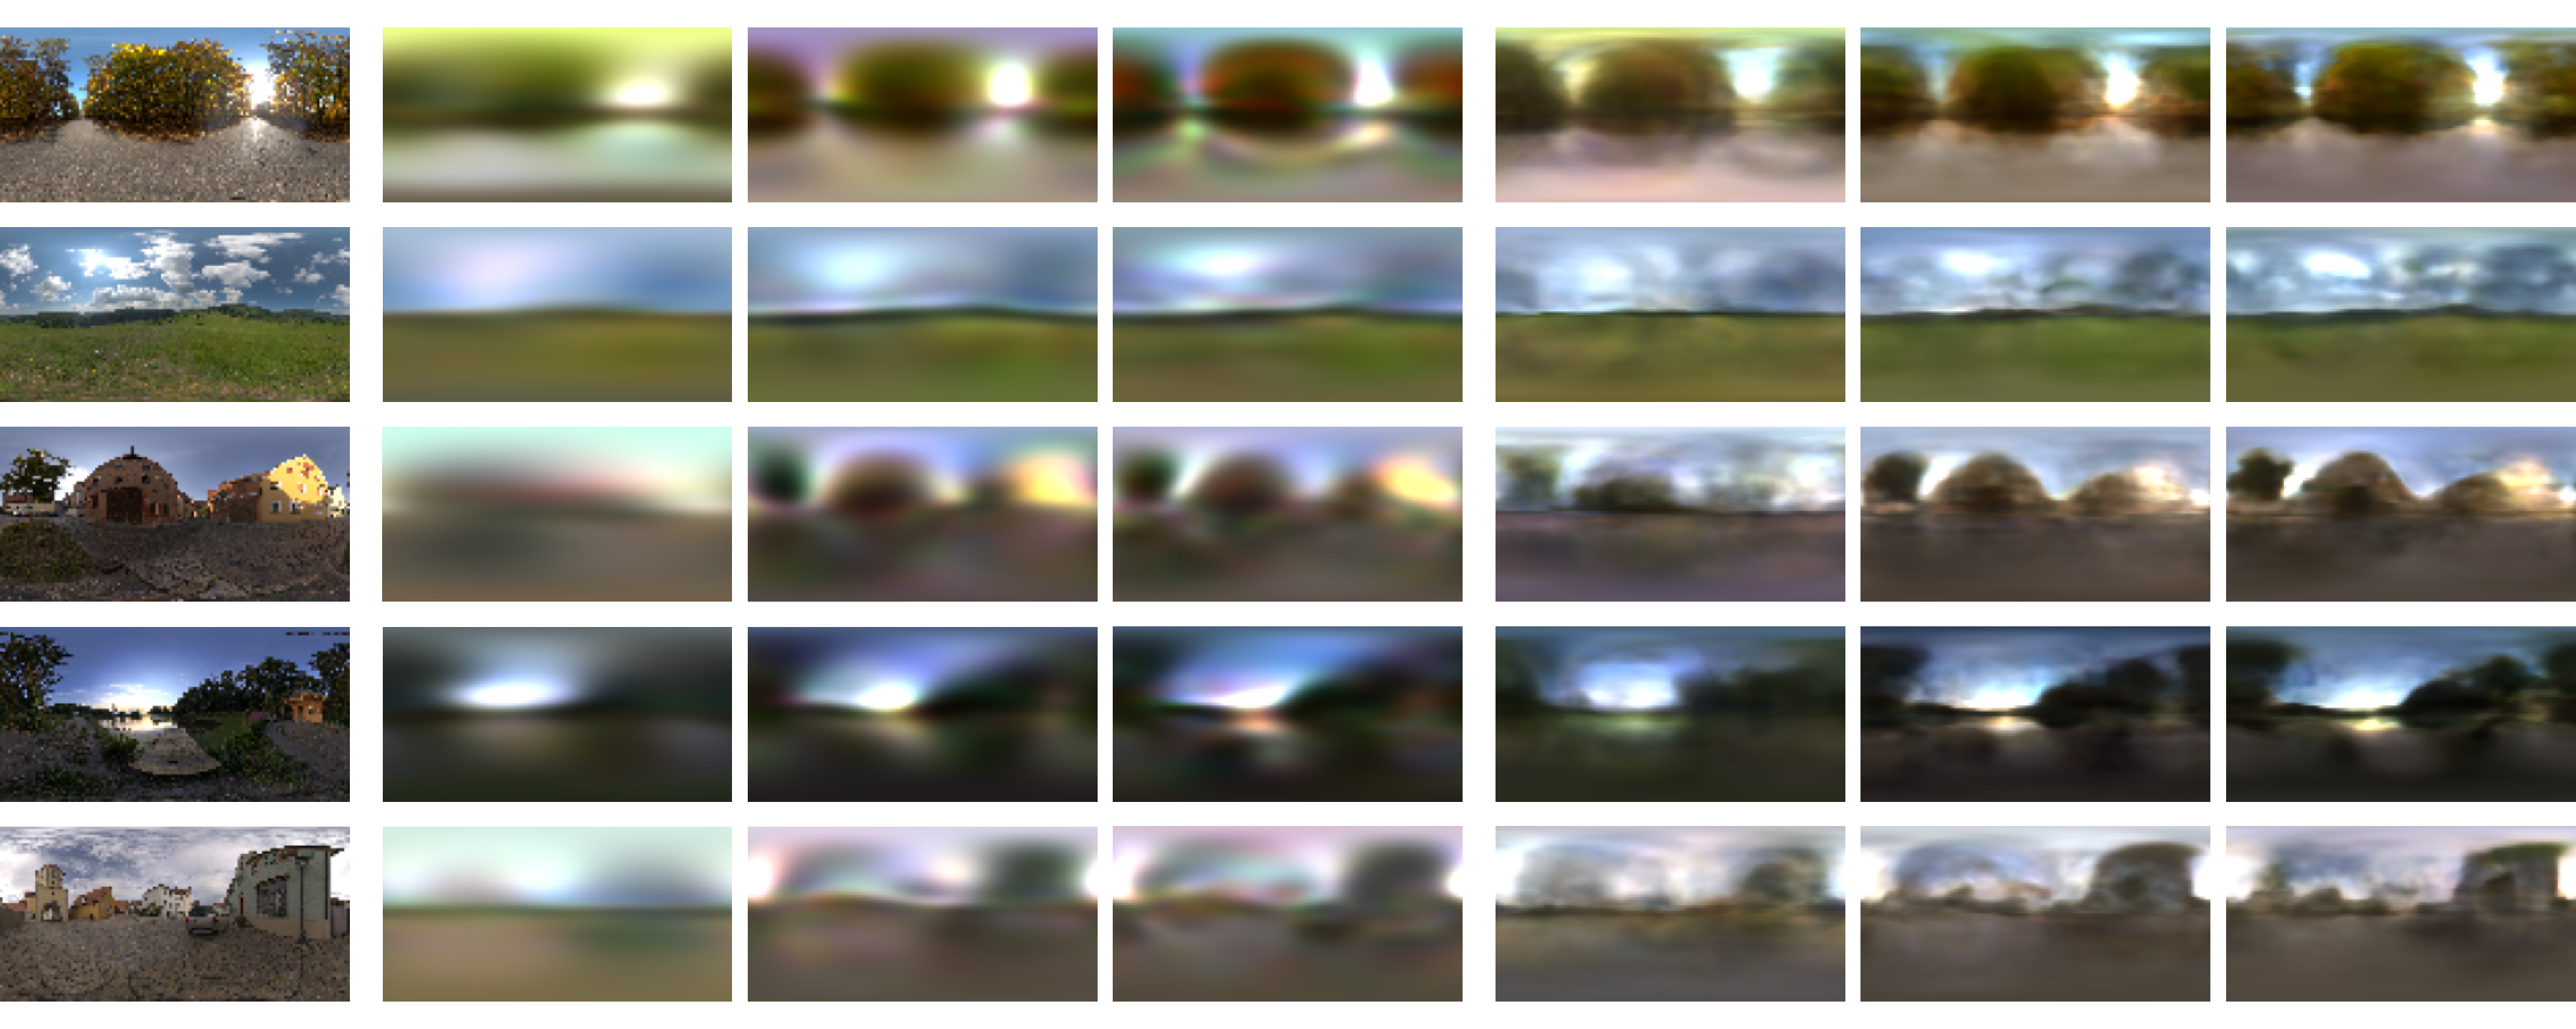
\includegraphics[width=0.98\textwidth]{Figures/old_vs_new.pdf}};
    \node at (-7.65, 3.95) {\small Ground};
    \node at (-7.65, 3.60) {\small Truth};
    \node at (-2.55, 3.95) {\small RENI};
    \node at (5.1, 3.95) {\small RENI++};
    \node at (-5.1, 3.60) {\small 27};
    \node at (-2.55, 3.60) {\small 147};
    \node at (0.0, 3.60) {\small 300};
    \node at (2.5, 3.60) {\small 27};
    \node at (5.0, 3.60) {\small 147};
    \node at (7.55, 3.60) {\small 300};
    \end{tikzpicture}
    \caption{A comparison between our prior RENI implementation and RENI++ for various latent dimensions. Col. $1$ shows the ground-truth environment map. Cols. $2-7$ shows prior RENI and RENI++ output for model sizes \(D = 27, 149, 300\).}
    \label{fig:old_vs_new}
\end{figure*}

\begin{table*}[h]
\centering
\ra{1.3}
\begin{tabular}{@{}cccc@{}}\toprule
\textbf{Rotation Angle (Degrees)} & \textbf{Relative Error} & \textbf{Ground Truth Rotation Matrix Error} \\ \midrule
5 & $0.582 \pm 0.140$ & $0.150 \pm 0.108$ \\
20 & $0.762 \pm 0.140$ & $0.243 \pm 0.123$ \\
45 & $0.838 \pm 0.098$ & $0.416 \pm 0.291$ \\
90 & $0.049 \pm 0.049$ & $0.008 \pm 0.009$ \\
180 & $0.050 \pm 0.045$ & $0.007 \pm 0.005$ \\
270 & $0.044 \pm 0.048$ & $0.006 \pm 0.005$ \\
\bottomrule
\end{tabular}
\caption{Mean relative error and rotation matrix discrepancy for optimised latent codes across various rotation angles of the test set.}
\label{tab:rotation_error_comparison}
\end{table*}

\begin{table*}\centering
\ra{1.3}
\begin{tabular}{@{}c c cc cc cc cc@{}}\toprule
& & \multicolumn{2}{c}{27} & \multicolumn{2}{c}{108} & \multicolumn{2}{c}{147} & \multicolumn{2}{c}{300}   \\
\cmidrule(lr){3-4} \cmidrule(lr){5-6} \cmidrule(lr){7-8} \cmidrule(lr){9-10}
Component & Training Steps & LDR & HDR & LDR & HDR & LDR & HDR & LDR & HDR \\
\midrule
RENI \cite{gardner2022rotation} & 4,015,200 & 17.02 & 32.70 & 19.58 & 33.63 & 19.97 & 33.78 & 20.47 & 34.03 \\
RENI retrained & 50,000 & 12.93 & 30.94 & 14.18 & 31.41 & 15.54 & 31.90 & 16.53 & 32.00 \\
w/ Transformer Decoder & 50,000 & 13.05 & 30.90 & 14.71 & 31.52 & 15.06 & 31.81 & 16.90 & 32.28 \\
+ Scale-Invariance (RENI++) & 50,000 & \textbf{18.02} & \textbf{33.00} & \textbf{20.87} & \textbf{34.30} & \textbf{21.13} & \textbf{34.60} & \textbf{22.10} & \textbf{35.10} \\
\bottomrule
\end{tabular}
\caption{Mean PSNR in Low Dynamic Range (LDR) and High Dynamic Range (HDR) on the test set for various ablations of the RENI++ architecture. ``RENI'' is the model architecture and weights directly from \cite{gardner2022rotation}, converted to work in Nerfstudio. ``RENI retrained'' is the same model but trained to match the number of steps used to train RENI++. The transformer decoder in RENI++ is sized to have a similar number of parameters as the SIREN-based condition-by-concatenation decoder. All results for models training within Nerfstudio are trained for $80\times$ fewer steps than the original RENI implementation. Despite this disadvantage, once Scale-Invariance is introduced, the Transformer Decoder outperforms RENI across all latent code sizes.}
\label{tab:ablation_study}
\end{table*}

\subsection{Inverse Rendering}
\label{Inverse Rendering} 

To test the performance of RENI++ in an inverse rendering pipeline, we implemented a normalised Blinn-Phong environment map shader within Nerfstudio, enabling fully differentiable rendering. We did not evaluate our model on the OpenIllumination dataset \cite{isabellaliulinghaochenOpenIlluminationMultiIlluminationDataset2023} due to its use of non-natural illumination conditions that RENI++ is not trained to represent. Instead, we render a 3D object with fixed geometry, pose, camera and material parameters such that only the lighting in the scene is unknown. Optimising only latent codes, we minimise Mean Squared Error and Cosine Similarity losses between a rendering using a ground truth environment map and one using the output of RENI++ or Spherical Harmonics. In the case of RENI++ we also include a prior loss on the latent codes:
\begin{equation}\label{inverse_loss}
    \mathcal{L}_{\text{Inverse}} = \rho \mathcal{L}_{\text{MSE}} + \gamma \mathcal{L}_{\text{Cosine}} + \beta \mathcal{L}_{\text{Prior}},
\end{equation}
where:
\begin{equation}\label{prior_loss}
    \mathcal{L}_{\text{prior}} = \frac{1}{K} \sum_{i=1}^K \left( \mathbf{Z}_i \right)^2,
\end{equation}
with $K$ being the number of unique latent codes in a batch.
This was tested for incremental increases in the weighting of the Blinn-Phong specular term $(K_{s})$, from $K_{s} = 0$ to $K_{s} = 1.0$ in steps of $0.2$. A normalisation factor \(\zeta = (n+2) / (4\pi(2-e(\frac{-n}{2})))\) \cite{gotanda_physically-based_2010}, was applied to $K_{s}$ to get a steady transition from diffuse to specular. We achieved the best performance using $\rho = 10^{2}$, $\gamma = 1.0$ and $\beta = 10^{-3}$, and a learning rate of \(10^{-2}\) for 200 steps. We use an environment map resolution of $H=64$ and render the object with a resolution of $128^{2}$. In Figure \ref{fig:inverse_rendering} we compare against SH environment maps implemented within Nerfstudio and optimise the SH parameters using the same inverse rendering pipeline as the RENI++ latent codes. RENI++ outperforms SH for all $K_{s}$ values whilst the prior ensures realistic and natural-looking environment estimations.

\subsection{Non-convexity of Reconstruction Error in Latent Space}
\label{Non-convexity} 
RENI++ is rotation equivariant. However, this does not necessarily mean that optimising to fit a rotated image will yield a rotated version of the latent code resulting from fitting to an unrotated version of the image. This means that the loss landscape of our reconstruction losses is not convex. To verify this, we fit RENI++ to versions of the test set at different rotations. Initialising at the mean environment and optimising resulted in sets of latent codes $\mathbf{Z}_\text{Rot}$ that we could compare to latent codes fit to the unrotated images  $\mathbf{Z}_\text{Un-rot}$. Ideally, this would result in each latent code being explained via a $y$-axis rotation of the other. To test this we minimised $\mathbf{M}$ for $\left \| \mathbf{Z}_\text{Un-rot}\mathbf{M} - \mathbf{Z}_\text{Rot}  \right \|_{2}$ and obtained a rotation matrix $\mathbf{R}$ that minimises $\left \| \mathbf{M} - \mathbf{R} \right \|_{F}$. We then calculate the relative error between $\mathbf{R}\mathbf{Z}_\text{Un-rot}$ and $\mathbf{Z}_\text{Rot}$: 
\[
E = \frac{\left \| \mathbf{R}\mathbf{Z}_\text{Un-rot} - \mathbf{Z}_\text{Rot} \right \|_{F}}{\left \| \mathbf{Z}_\text{Rot} \right \|_{F}}.
\]

The results are shown in Table. \ref{tab:rotation_error_comparison}. For the rotations of $90$, $180$, and $270$ degrees, the relative error is very small demonstrating that both latent codes can largely be explained as a simple rotation of the other. However, for the remaining three smaller rotations the error was higher, suggesting there is redundancy in the latent space, i.e. there are multiple possible explanations for a single image. Better latent space regularisation, tuning model dimensionality and a larger dataset might help resolve this.


\subsection{Reflection Equivariance}

In Figure \ref{fig:mirror} we visually illustrate the expected reflection equivariance of our model. We generate a random latent code representing a random, natural illumination environment (top). Since our model is equivariant to reflections about any plane parallel to the rotation axis $\mathbf{a}=\mathbf{e}_y$, we show that reflections of the latent code about the $x=0$ and $z=0$ planes results in a corresponding reflection of the environment about those planes (bottom left and right). However, the model is not equivariant to reflections about the $y=0$ plane (which would result in environments with the sky at the bottom). So, reflections of the latent code about the $y=0$ plane (bottom middle) results in an entirely new environment, unrelated to the original one.

\begin{figure}
    \centering
    \makebox[\columnwidth]{%
        \begin{tikzpicture}
        \node (img) {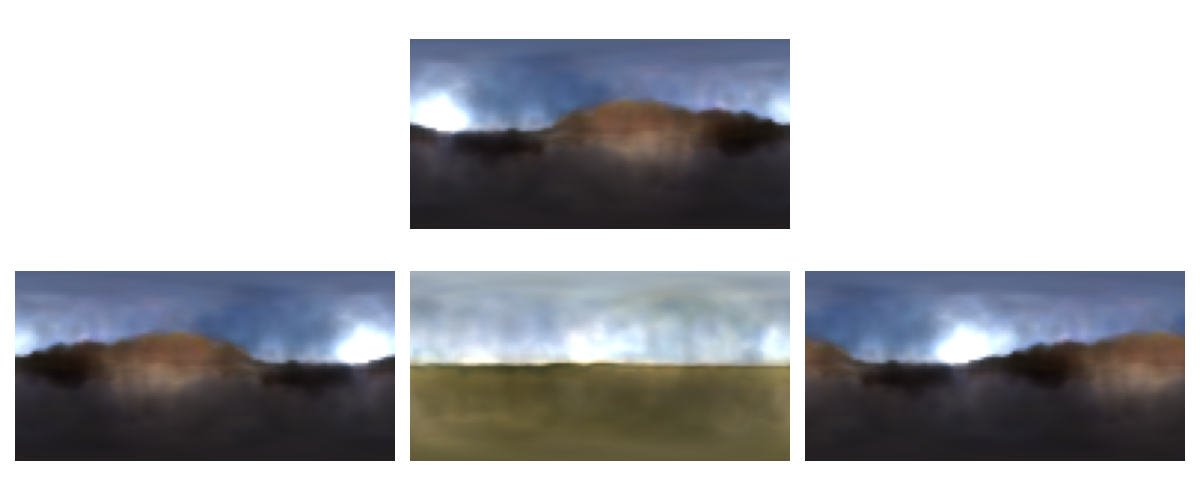
\includegraphics[width=0.98\columnwidth]{Figures/mirror.png}};
        \node at (0.0, 1.7) {\scriptsize $\mathbf{Z}$};
        \node at (-2.85, -0.01) {\scriptsize $\text{diag}(-1,1,1)\mathbf{Z}$};
        \node at (0.0, -0.01) {\scriptsize $\text{diag}(1,-1,1)\mathbf{Z}$};
        \node at (2.85, -0.01) {\scriptsize $\text{diag}(1,1,-1)\mathbf{Z}$};
        \end{tikzpicture}
    }
    \caption{Our model is $O(2)$-equivariant to reflections about the $x=0$ and $z=0$ planes. Hence, reflections of the latent codes exactly correspond to reflections of the illumination environment. However, reflections about the $y=0$ plane represent an entirely different illumination condition.}
    \label{fig:mirror}
\end{figure}


\begin{sidewaysfigure*}
  \centering
  \makebox[\textwidth]{%
      \begin{tikzpicture}
        \newcommand\smallermath{\fontsize{4pt}{5pt}\selectfont}
        \node (img) {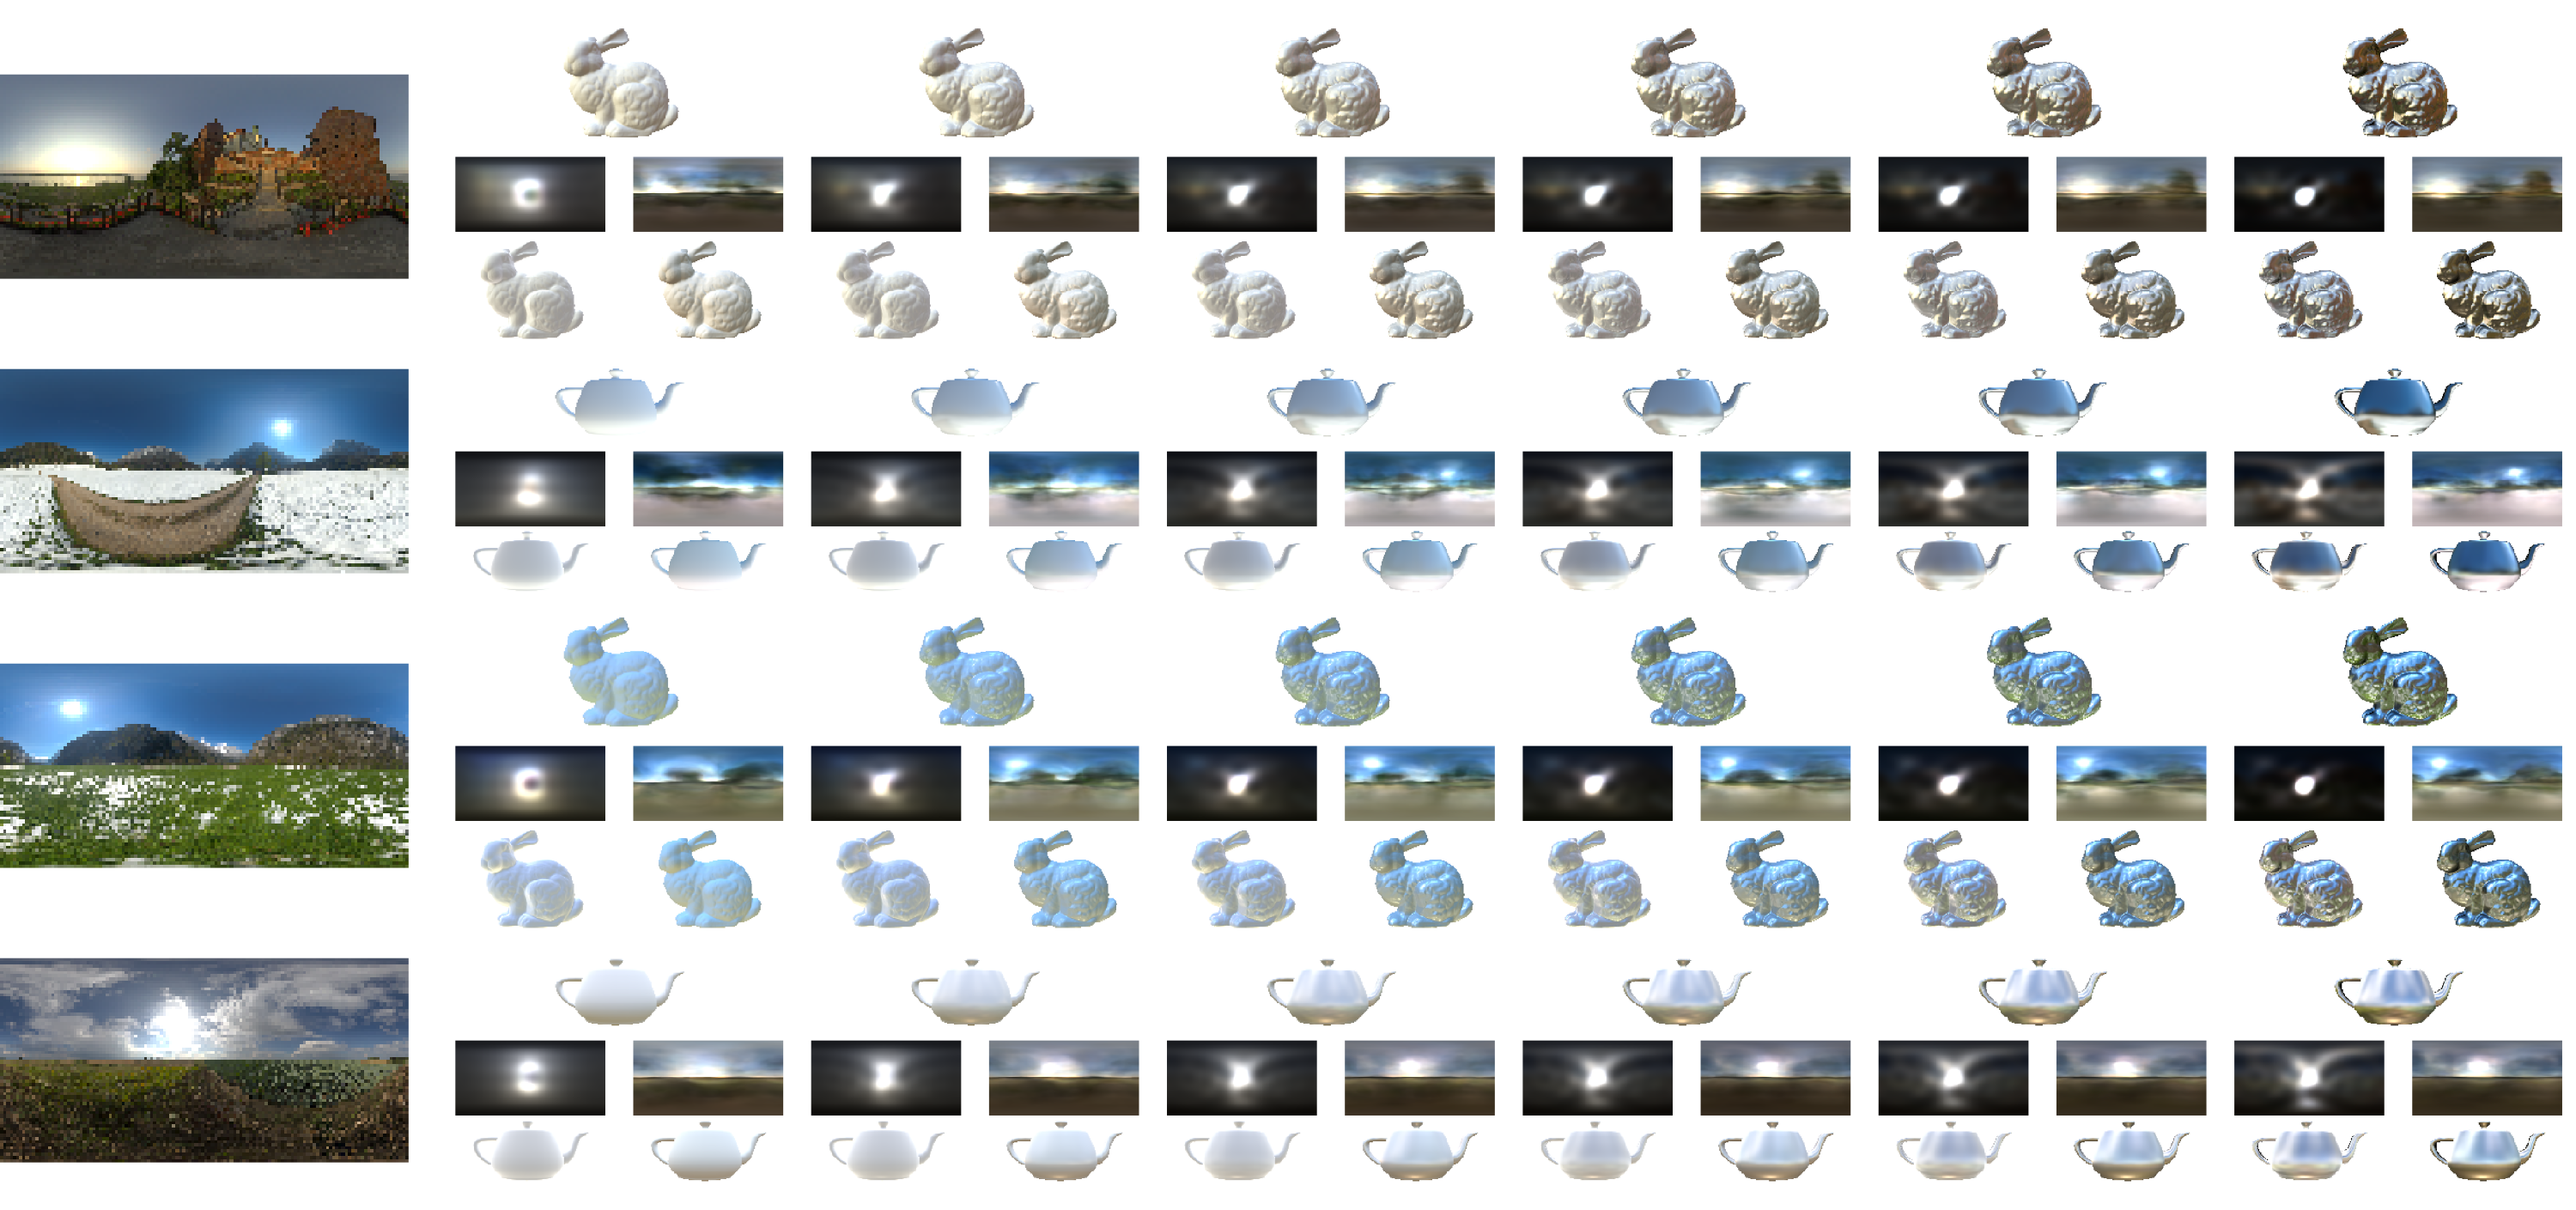
\includegraphics[width=\textwidth]{Figures/inverse_rendering.png}};
        \node at (-10.4, 5.7) {\small Ground Truth};
        \node at (-10.4, 5.4) {\small Environment Map};
        \node[rotate=90, font=\scriptsize] at (-8.15, 4.97) {Target};
        \node[rotate=90, font=\scriptsize] at (-8.202, 3.95) {Recon};
        \node[rotate=90, font=\scriptsize] at (-8.2, 3.14) {Fit};
        
        \node[rotate=90, font=\scriptsize] at (-8.15, 1.86) {Target};
        \node[rotate=90, font=\scriptsize] at (-8.202, 1.11) {Recon};
        \node[rotate=90, font=\scriptsize] at (-8.2, 0.36) {Fit};
        
        \node[rotate=90, font=\scriptsize] at (-8.15, -0.75) {Target};
        \node[rotate=90, font=\scriptsize] at (-8.202, -1.73) {Recon};
        \node[rotate=90, font=\scriptsize] at (-8.2, -2.65) {Fit};
        
        \node[rotate=90, font=\scriptsize] at (-8.15, -3.8) {Target};
        \node[rotate=90, font=\scriptsize] at (-8.202, -4.55) {Recon};
        \node[rotate=90, font=\scriptsize] at (-8.2, -5.3) {Fit};
    
        \node[font=\small] at (1.5, 6.1) {Increasing Specularity};
        
        \draw[->] (-5.8,5.9) -- (8.8,5.9); % Draws a line with an arrow at the end
    
        \node[font=\scriptsize] at (-6.45, 5.7) {0.0};
        \node[font=\scriptsize] at (-3.05, 5.7) {0.2};
        \node[font=\scriptsize] at (0.41, 5.7) {0.4};
        \node[font=\scriptsize] at (3.83, 5.7) {0.6};
        \node[font=\scriptsize] at (7.3, 5.7) {0.8};
        \node[font=\scriptsize] at (10.7, 5.7) {1.0};
    
        % For 0.0
        \node[font=\scriptsize] at (-7.3, 4.46) {SH};
        \node[font=\scriptsize] at (-5.55, 4.46) {RENI++};
        
        % For 0.2
        \node[font=\scriptsize] at (-3.9, 4.46) {SH};
        \node[font=\scriptsize] at (-2.10, 4.46) {RENI++};
        
        % For 0.4
        \node[font=\scriptsize] at (-0.44, 4.46) {SH};
        \node[font=\scriptsize] at (1.31, 4.46) {RENI++};
        
        % For 0.6
        \node[font=\scriptsize] at (2.98, 4.46) {SH};
        \node[font=\scriptsize] at (4.73, 4.46) {RENI++};
        
        % For 0.8
        \node[font=\scriptsize] at (6.40, 4.46) {SH};
        \node[font=\scriptsize] at (8.2, 4.46) {RENI++};
        
        % For 1.0
        \node[font=\scriptsize] at (9.80, 4.46) {SH};
        \node[font=\scriptsize] at (11.6, 4.46) {RENI++};
    
        
      \end{tikzpicture}
  }
  \caption{Reconstruction results in an inverse rendering task. The specular Blinn-Phong term $K_{s}$ increases from left to right in steps of $0.2$. Both RENI++ and SH have a dimensionality of $D = 300$. RENI++ outperforms SH across all $K_{s}$ and as $K_{s}$ increases the environments predicted by RENI++ become significantly more detailed and accurate.}
  \label{fig:inverse_rendering}
\end{sidewaysfigure*}